
% Eigener Beitrag: Beschreibung, Begründung, Aufzeigung, Methode, Fazit

\chapter{Anforderungen und Analyse}
\label{sec:analyse}
Es gibt folgende Anforderungen an die Testsuite:
\begin{figure}[H]
	\centering
	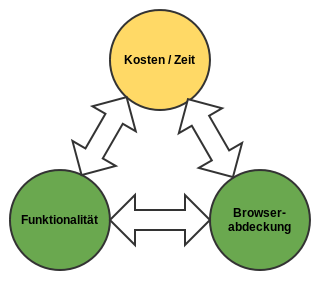
\includegraphics[width=0.6\textwidth]{images/triangle.png}
	\caption{Anforderungsdreieck}
	\label{fig:analyse:Anforderungsdreieck}
\end{figure}

Kosten \& Zeit sind wichtig, da die Tests oft gestartet werden müssen und deshalb nicht zu lange dauern sollten. Und bei den Serviceanbietern Saucelabs und CrossBrowserTesting zahlt man für die Zeit wie lange die Tests dauern.

Je mehr Funktionalität abgedeckt wird, desto länger dauern die Test. Und für jeden Browser müssen nochmals alle Tests durchgeführt werden. 

Deshalb stehen Kosten / Zeit im Widerspruch mit Funktionalität und der Browserabdeckung.

Diese Anforderungen sind in den nächsten Abschnitten beschrieben.

\section{Funktionalität}
Die gesamte Funktionalität der Webseite ist im \cref{app:A} \nameref{app:A} aufgelistet. Die Liste wurde im Wiki von der Hotelplan Management AG erstellt. Diese soll auch nach der Arbeit weiter gepflegt werden und wurde deshalb so aufgebaut, dass sie sehr Übersichtlich ist und einfach bearbeitet und erweitert werden kann.

\section{Browserabdeckung}
Im \cref{sec:Recherche:TestingFrameworks:Prototyp} \nameref{sec:Recherche:TestingFrameworks:Prototyp} sind die meist verwendeten Browser aufgelistet. Der Vorteil an den Serviceanbietern ist, dass es sehr leicht ist eine Testsuite auf einem weiteren Webbrowser auszuführen. Es ist zu eruieren wie lange die Tests brauchen um durchzulaufen. Dann kann entschieden werden, im Betracht der Kosten, auf wie vielen Browsern die Testsuite durchgeführt wird.

\section{Kosten \& Zeit}
Wie bereits erwähnt wird bei den Serviceanbieter pro Minute abgerechnet, die die Tests benötigen. Und für jeden Test wird eine neue \Gls{glos:virtualMachine} gestartet, was zusätzliche Zeit braucht. Deshalb wird versucht, die Anzahl der Testfälle zu minimieren, um trotzdem die gesamte Funktionalität abdecken zu können.

Je nachdem wie lange die Tests benötigen kann über die Anzahl der Browser, auf denen die Tests laufen gelassen werden, die Kosten gesteuert werden.